\documentclass{article}
\usepackage{graphicx}
\usepackage{booktabs}
\title{Comprehensive System Walkthrough Manuscript}
\author{QA Benchmark Author}
\begin{document}
\maketitle

\section{Basic Writing}
this paragraph is very bad and i write like chat message, it do not have proper grammar and the logic are broken and the transition are messy.
we was trying many random settings and maybe it works maybe not, anyway this sentence is too long and it keeps going without clear structure and it sounds informal.

\section{Text-Table Mismatch}
Table 1 shows our accuracy is 95\%.
\begin{table}[t]
\centering
\caption{Main Evaluation Result}
\label{tab:main}
\begin{tabular}{lcc}
\toprule
Metric & Baseline & Ours \\
\midrule
Accuracy & 82\% & 88\% \\
\bottomrule
\end{tabular}
\end{table}

\section{Text-Figure Mismatch}
As shown in Figure~\ref{fig:loss} (Figure 1), the loss INCREASES over time and reaches 0.90.
\begin{figure}[t]
\centering
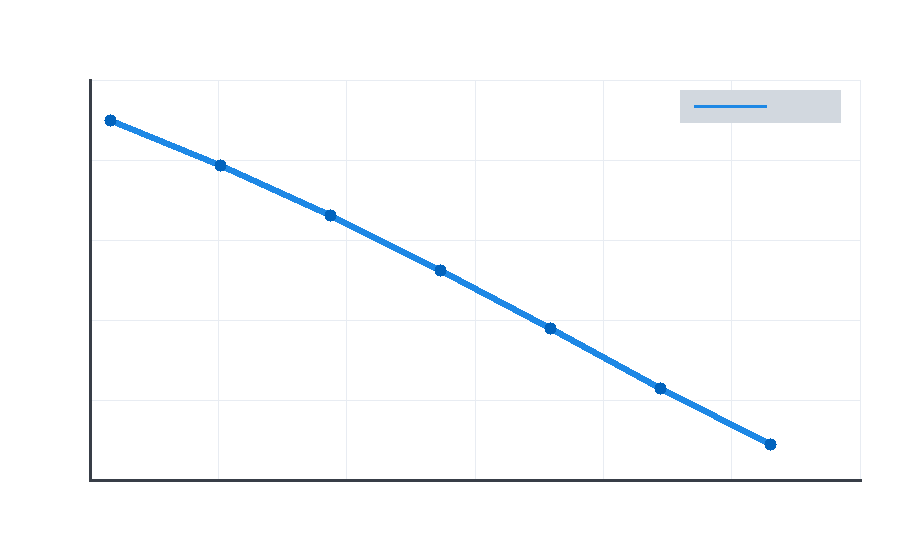
\includegraphics[width=0.60\linewidth]{dummy_plot.png}
\caption{Loss over Epochs}
\label{fig:loss}
\end{figure}

\section{Citation Hallucination}
Prior work \cite{Fake2099} proved this result with absolute certainty.

\section{Terminology}
Our method is based on a Large Language Model architecture. Later we abbreviate it as LLM for convenience.
In the ablation discussion we also call it a Large-scale Language Model, which may confuse terminology consistency.

\bibliography{references}
\bibliographystyle{plain}
\end{document}
